\documentclass[tikz,border=4pt]{standalone}
\usepackage{tikz}
\usetikzlibrary{arrows.meta}
\begin{document}
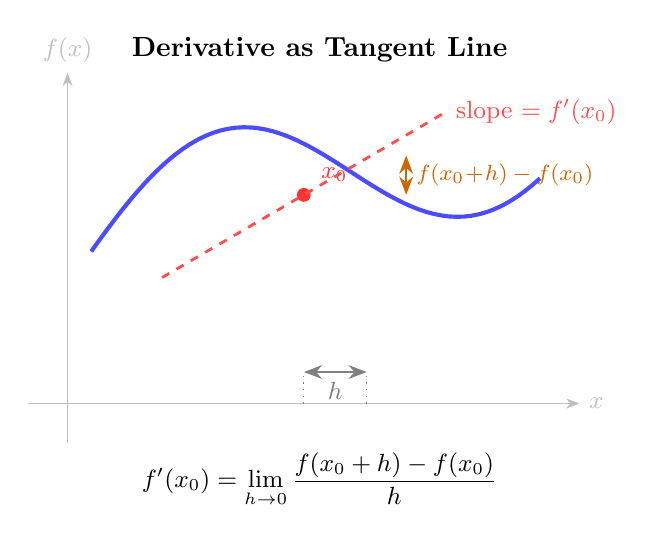
\begin{tikzpicture}[>=Stealth]
    \node[font=\bfseries] at (3.2,4.5) {Derivative as Tangent Line};

    % Axes
    \draw[->,gray!50] (-0.5,0) -- (6.5,0) node[right,font=\small] {$x$};
    \draw[->,gray!50] (0,-0.5) -- (0,4.2) node[above,font=\small] {$f(x)$};

    % Curve
    \draw[blue!70,line width=1.5pt,domain=0.3:6,samples=60]
        plot ({\x},{1.5+1.2*sin(50*\x)+0.4*\x});

    % Point of tangency
    \fill[red!80] (3,2.65) circle (2.5pt);
    \node[red!80,font=\small,above right] at (3.1,2.7) {$x_0$};

    % Tangent line
    \draw[red!70,line width=1pt,dashed] (1.2,1.6) -- (4.8,3.7)
        node[right,font=\small,red!70] {slope $= f'(x_0)$};

    % h annotation
    \draw[<->,gray,line width=0.8pt] (3,0.4) -- (3.8,0.4)
        node[midway,below,font=\small] {$h$};
    \draw[dotted,gray] (3,0) -- (3,0.4);
    \draw[dotted,gray] (3.8,0) -- (3.8,0.4);

    % f(x+h) - f(x) annotation
    \draw[<->,orange!80!black,line width=0.8pt] (4.3,2.65) -- (4.3,3.15)
        node[midway,right,font=\footnotesize] {$f(x_0\!+\!h)-f(x_0)$};

    % Formula
    \node[font=\small,anchor=north] at (3.2,-0.5)
        {$f'(x_0)=\displaystyle\lim_{h\to 0}\frac{f(x_0+h)-f(x_0)}{h}$};
\end{tikzpicture}
\end{document}
